\section{Zielsetzung}
Ziel dieses Versuches ist es, die Fresnelschen Formeln zu verifizieren, indem 
ein Laserstrahl an einem Siliziumkristall gebrochen wird.
Außerdem soll ein experimenteller Wert des Brechungsindex von Silizium sowie der
Brewsterwinkel bestimmt werden.

\section{Theorie}
\label{sec:Theorie}
Licht, welches aus einem Medium in ein anderes übergeht, wird an der Grenzfläche
zwischen den Medien gebrochen und reflektiert.
Für den transmittierten Teil gilt des Snelliussche Brechungsgesetz
\begin{equation}
    n_1\sin(\alpha) = n_2 \sin{\beta}. \label{eq:snellius}
\end{equation}
Dabei wird klar, dass die Brechung in direktem Zusammenhang zu dem Einfallswinkel
und dem Verhältnis der Brechungsindices steht.

Zur näheren Beschreibung der Reflexion und Transmission von Licht werden die Fresnelschen Formeln hergeleitet.

\subsection{Herleitung der Fresnelschen Formeln}
Aufgrund der Tatsache, dass Licht aus elektromagnetischer Strahlung besteht, lässt sich die 
Strahlleistung mit dem Pointingvektor
\begin{equation*}
    \symbf{S} = \symbf{E} \times \symbf{H}
    \label{eq:Pointing}
\end{equation*}
schreiben. Mithilfe der Maxwellgleichungen der Elektrodynamik lässt sich der Betrag des 
Pointingvektors~\eqref{eq:Pointing} zu
\begin{equation}
    S = |\symbf{S}| = c \varepsilon \varepsilon_0 \symbf{E}^2
    \label{eq:Pointingbetrag}
\end{equation}
berechnen. Mit Energieüberlegungen und dem Betrag des Pointingvektors~\eqref{eq:Pointingbetrag} kann
die Aufteilung der Strahlleistung 
\begin{equation}
    S_{\text{ein}} \cos(\alpha) = S_{\text{ref}} \cos(\alpha) + S_{\text{trans}} \cos(\beta)
    \label{eq:Aufteilung}
\end{equation}
bestimmt werden. Die geometrischen Überlegungen dazu sind in \autoref{fig:Reflexion} dargestellt.
\begin{figure}[H]
    \centering
    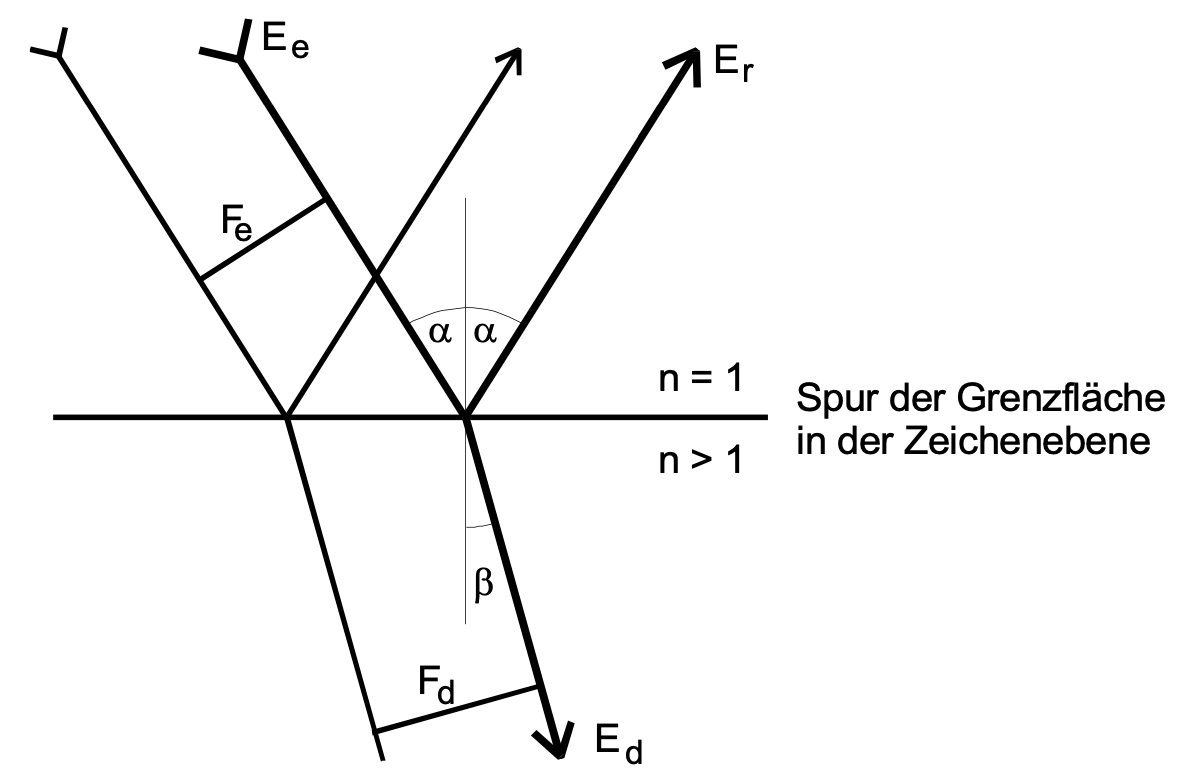
\includegraphics[height=6cm]{content/pics/Reflexion.png}
    \caption{Skizzierung von Reflexion und Brechung an einer Grenzfläche \cite{v407}.}
    \label{fig:Reflexion}
\end{figure}
Wird der Betrag des Pointingvektor~\eqref{eq:Pointingbetrag} in die Aufteilung~\eqref{eq:Aufteilung} 
eingesetzt, ergibt sich
\begin{equation}
    (\symbf{E}_{\text{ein}}^2 - \symbf{E}_{\text{ref}}^2)\cos(\alpha) = n \symbf{E}_{\text{trans}}^2 \cos(\beta).
\end{equation}
Dafür wird $n^2=\varepsilon$ und $c^2 = (\varepsilon \varepsilon_0 \mu_0)^{-1}$, was für nicht-ferromagnetische
Stoffe gilt, verwendet.
Das elektrische Feld lässt sich in einen senkrecht parallel polarisierten Teil gemäß
\begin{equation*}
    \symbf{E} = \symbf{E}_{\symup{s}} + \symbf{E}_{\symup{p}}
\end{equation*}
aufteilen. Mithilfe von Stetigkeitsüberlegungen 
\begin{align*}
    \symbf{E}_{\text{ein}, s} + \symbf{E}_{\text{ref}, s} &= \symbf{E}_{\text{trans}, s} \\
    (\symbf{E}_{\text{ein}, p} - \symbf{E}_{\text{ref}, p})\cos(\alpha) &= \symbf{E}_{\text{trans}, p} \cos(\beta)
\end{align*}
an der Grenzfläche lässt sich $\symbf{E}_{\text{trans}}$ herauskürzen. Wird darüber hinaus das Snelliussche
Brechungsgesetz~\eqref{eq:snellius} eingesetzt, ergibt sich für die s- und p-polarisierten Amplituden des 
$\symbf{E}$-Feldes zu
\begin{align}
    \symbf{E}_{\text{ref, s}} &= -\symbf{E}_{\text{ein, s}} \cdot \frac{\sqrt{n^2-\sin^2(\alpha)}-\cos(\alpha)}{n^2-1}
    \label{eq:Fresnel s} \\
    \symbf{E}_{\text{ref, p}} &= \symbf{E}_{\text{ein, p}} \cdot \frac{n^2 \cos(\alpha) - \sqrt{n^2-\sin^2(\alpha)}}{n^2 \cos(\alpha) + \sqrt{n^2-\sin^2(\alpha)}}.
    \label{eq:Fresnel p}
\end{align}

\subsection{Brewsterwinkel}
Der Brewsterwinkel $\alpha_{\symup{p}}$ beschreibt den Winkel, unter dem ein Lichtstrahl vollständig durch
eine Grenzfläche transmittiert, also der reflektierte Anteil verschwindet. Er ergibt sich, indem 
Gleichung~\eqref{eq:Fresnel p} mit Additionstheoremen zu
\begin{equation*}
    \symbf{E}_{\text{ref, p}} = \symbf{E}_{\text{ein, p}} \cdot \frac{\tan(\alpha-\beta)}{\tan(\alpha+\beta)}
\end{equation*}
umgeschrieben wird. Für ein 
\begin{equation}
    \alpha_{\symup{p}}+\beta_{\symup{p}}=\frac{\symup{\pi}}{2}
    \label{eq:herleitung brewster}
\end{equation}
gilt $\tan(\frac{\symup{\pi}}{2}) \to \infty$, 
weshalb der gesamte Term null wird. Die Bedingung~\eqref{eq:herleitung brewster} wird in das Snelliussche
Brechungsgesetz~\eqref{eq:snellius} eingesetzt und es folgt
\begin{equation}
    n_2 = \tan(\alpha_p),
    \label{eq:Brewsterwinkel}
\end{equation}
wenn der Brechungsindex für Luft mit $n_1\approx 1$ approximiert wird.